\documentclass[
  leqno, % 数式左詰め
  twoside, % 両開き
  numbers=noenddot, % 節番号の末尾に.を付けない
  headsepline, % ヘッダ線あり
  footsepline, % フッタ線あり
]{scrbook}
\usepackage{luatexja-preset} % 日本語化
%\usepackage[hiragino-pron]{luatexja-preset} % 日本語化(macOS用)
\usepackage[main=japanese,english]{babel} % 用語の日本語化
\makeatletter % 章の表記を変えたい場合はここから
\renewcommand{\chapterlinesformat}[3]{%
  \renewcommand*{\thechapter}{{第}\@arabic\c@chapter{章}}
  \@hangfrom{#2}{#3}%
}
\makeatother % ここまでを使う
\usepackage[ % 
  bottom=40mm, % 下側の空白の指定
  margin=30mm, % 左右の空白の指定
  showframe=false, % 本文の領域を見る場合はtrue
]{geometry}
\usepackage[%
  backend=biber,
  bibencoding=latin1,
  style=ieee, % ieee, nature, numeric, authoryear いろいろある
  url=false, % 余計な項目は表示しない
  isbn=false,
  doi=false,
  eprint=false,
]{biblatex}
\AtEveryBibitem{\clearfield{note}} % note項目を表示しない
\addbibresource{papers.bib}
% \addbibresource{books.bib} % databaseを追加する場合

%%% 必要なpackageの読み込みの例
\usepackage{graphicx}
\graphicspath{{./imgs/}}
\usepackage{pdfpages}
\usepackage[
  bookmarks=true,%
  bookmarksnumbered=true,%
  colorlinks=true,%
  linkcolor=blue,%
  citecolor=blue,
  setpagesize=false]{hyperref}
\usepackage{amsmath,amssymb}
\usepackage[fleqn,tbtags]{mathtools} % amsmathの拡張
\mathtoolsset{showonlyrefs,showmanualtags} % ラベルありの数式のみ番号あり
\usepackage{bxjalipsum} % ダミーの文書
\usepackage[math]{blindtext} % ダミーの文書
%%% packageの例の終わり

%%% タイトル
\subject{2020年度修士論文}
\title{「我輩」の秘密に関する研究}
\subtitle{私が彼について知っている2,3の事柄} 
\author{夏目 漱石}
\date{\today}
\publishers{
  早稲田大学 先進理工学研究科\\
  電気・情報生命専攻\\
  情報学習システム研究室
}

%%% 本文
\begin{document}
\frontmatter
\maketitle
%% 概要書の読み込み
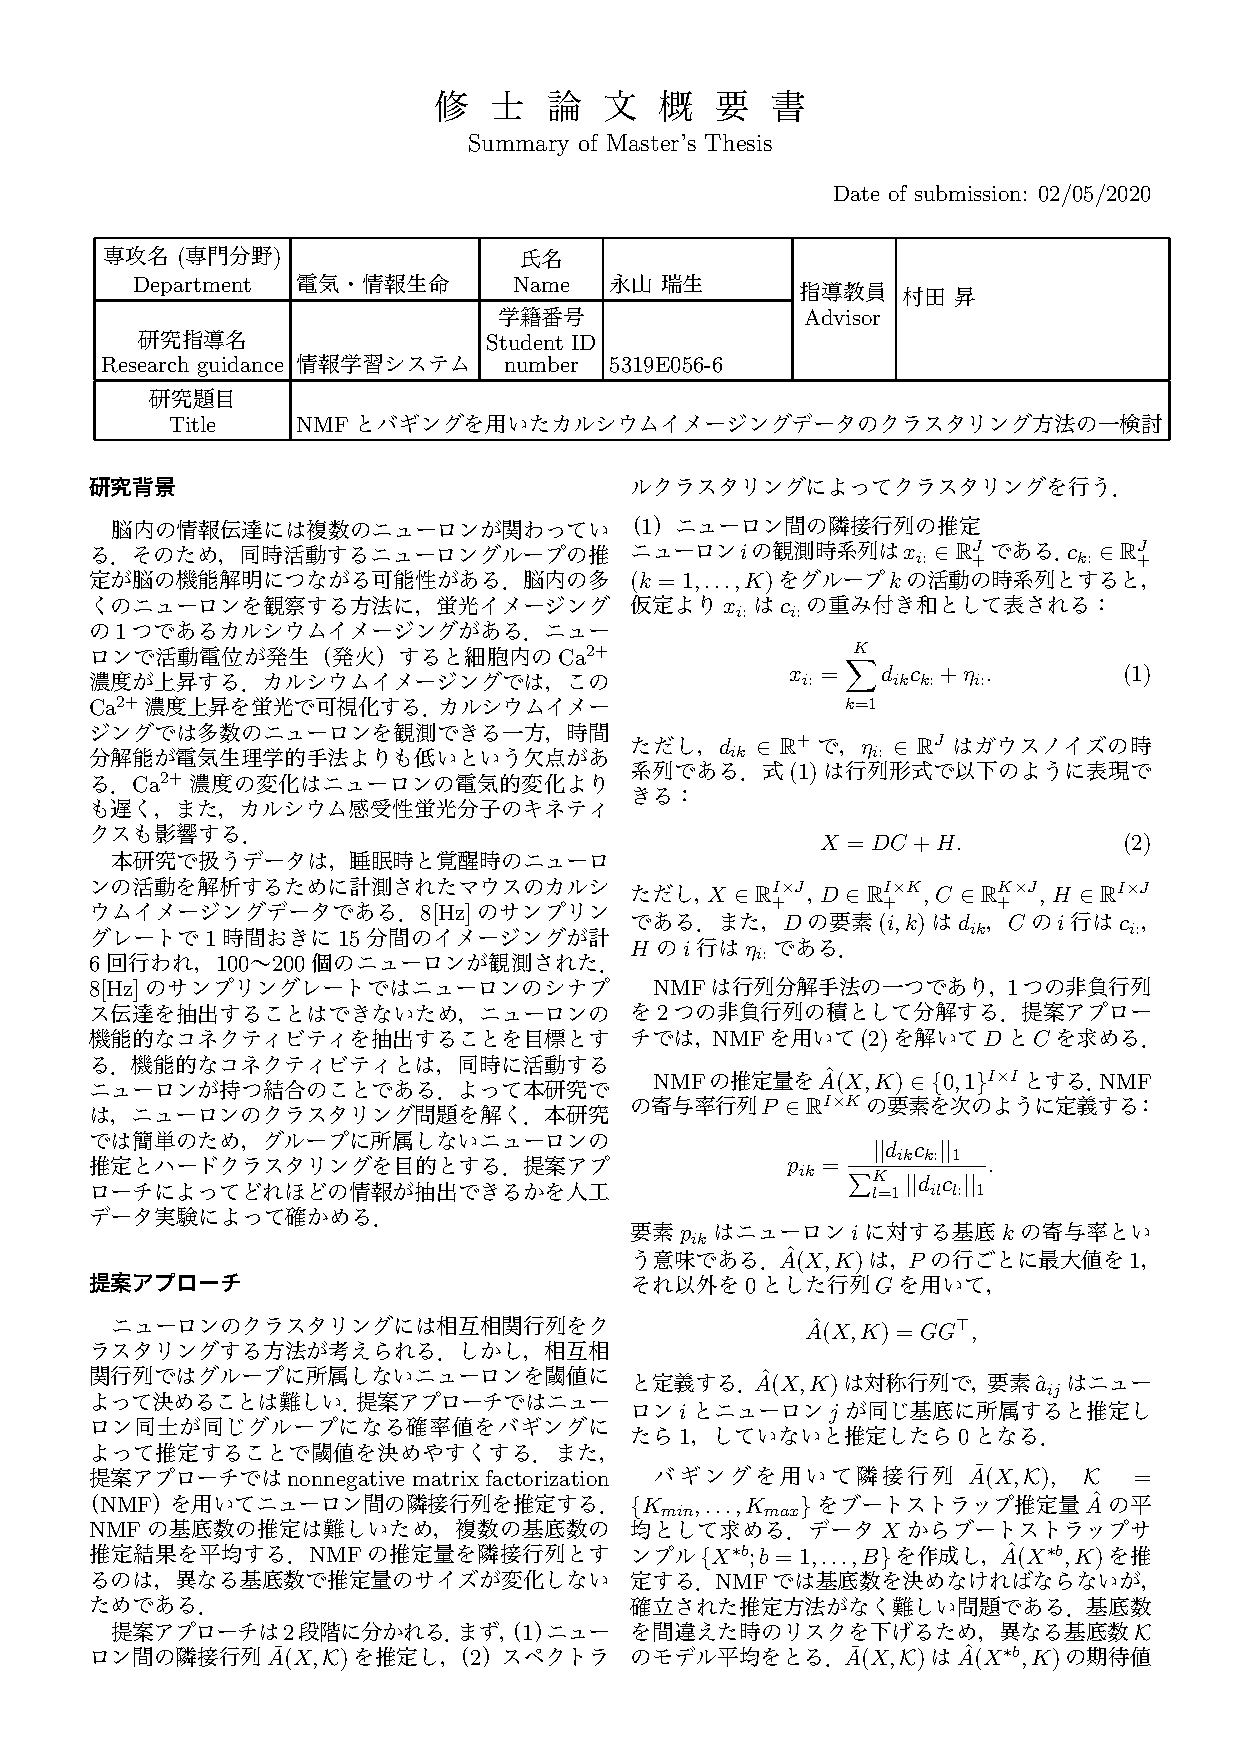
\includepdf[pages=-]{abstract.pdf}
%% ここまで
\tableofcontents

\mainmatter
%%% 以下本文の例
\chapter{はじめに}
\jalipsum{iroha}
\cite{Sonoda2017233,Hino20171838}

\chapter{問題設定}
\section{わがはい}
\jalipsum{wagahai}
\section{かどがたつ}
\jalipsum{kusamakura}
\cite{Kato2017115,Kato2016}

\chapter{提案手法}
\section{まえおき}
\jalipsum{preamble}
\section{数式はどうなるのか}
\blindmathpaper 
\cite{Chiba2017}

\chapter{応用例}
\jalipsum{hatsukoi}
\cite{Takano20162687,Koshijima20161560,Akaho2016}

\chapter{まとめ}
\jalipsum{jugemu}
%% 実際に各章は include すればよい
%% \include{1_Introduction} 

\backmatter
\begin{otherlanguage}{english}
  % babel-japaneseが若干悪さをするので英語にして回避
  \printbibliography[title=参考文献]
\end{otherlanguage}
\end{document}